\documentclass{beamer}

\usepackage{subfigure}
\usepackage{graphicx}
\usepackage{amsfonts}
\usepackage{amsmath}
\usepackage{amsthm}
\usepackage{wrapfig}
\usepackage{amssymb}

\makeatletter
\def\handoutsmode{handoutsmode}
\def\notesmode{notesmode}
\ifx\modetype\handoutsmode
  % Handouts mode: supress overlays
  \gdef\beamer@currentmode{handout}
\else\relax\fi
\ifx\modetype\notesmode
  % Notes mode: show notes and suppress overlays
  \gdef\beamer@currentmode{handout}
  \setbeameroption{show notes}
\else\relax\fi
\makeatother

% -- BEAMER PACKAGES & OPTIONS --
 \setbeamersize{text margin  left=.5cm}   % Default 1cm
 \setbeamersize{text margin right=.5cm}   % Default 1cm
 \usefonttheme[onlymath]{serif}           % Serif math font
 \setbeamertemplate{itemize items}[circle]
 \setbeamertemplate{section in toc}[sections numbered]
 \setbeamertemplate{navigation symbols}{} % No navigation symbols
%\setbeamercovered{invisible}             % Shadowed/invisible overlays
%\setbeameroption{show notes}
 \setbeamercolor{frametitle}{fg=black}
 \setbeamerfont{frametitle}{size=\large,series=\bfseries}
 \setbeamertemplate{frametitle}
 {
   \begin{centering}
     \insertframetitle\par
   \end{centering}
 }
% \setbeamertemplate{footline}[page number]  % Simple n/N footer
 \setbeamertemplate{footline}[text line]{%
   \vbox{%
%     \tinycolouredline{black}{\color{white}\bf%
       \insertpart\hfill%
       \insertpartnumber--\insertframenumber%
       \smallskip
 }}

% -- PACKAGES --
\usepackage{amsmath,amssymb,amsfonts}
\usepackage{bbding}
\usepackage{pstricks}

\usepackage[misc]{ifsym}
\usepackage{braket}
\usepackage{boxedminipage}
\usepackage{overpic}
% -- SLIDE MACROS --
\def\bc{\begin{center}}
%\def\be{\begin{enumerate}}
\def\bi{\begin{itemize}}
\def\bs{\begin{small}}
\def\ec{\end{center}}
%\def\ee{\end{enumerate}}
\def\ei{\end{itemize}}
\def\es{\end{small}}


% -- ONE-LINE SLIDES --
\newcommand{\TOPIC}[1]{
  \frame{LARGE\textbf{%
      \begin{center}
        \gr{#1}
      \end{center}}}}

% -- BOXED EQUATIONS --
%\usepackage{empheq}
\newenvironment{boxedeq}%
  {\begin{empheq}[box=\fbox]{align}}
  {\end{empheq}}

% -- MISC --
\newcommand{\com}[1]{\texttt{#1}}
\newcommand{\DIV}{\ensuremath{\mathop{\mathbf{DIV}}}}
\newcommand{\GRAD}{\ensuremath{\mathop{\mathbf{GRAD}}}}
\newcommand{\CURL}{\ensuremath{\mathop{\mathbf{CURL}}}}
\newcommand{\CURLt}{\ensuremath{\mathop{\overline{\mathbf{CURL}}}}}
\newcommand{\nullspace}{\ensuremath{\mathop{\mathrm{null}}}}
\newcommand{\BALL}{{\color{structure}$\bullet \;$}}
\newcommand{\eq}{\ =}
\newcommand{\plus}{\ +}
\newcommand{\footbar}{\hspace*{-2.5ex}\rule{2in}{.2pt}\\}
\newcommand{\topline}{\hrulefill}
\newcommand{\botline}{\vspace*{-1ex}\hrulefill}
\renewcommand{\emph}[1]{\textbf{#1}}
\newcommand{\mcol}[3]{\multicolumn{#1}{#2}{#3}}
\newcommand{\assign}{\ensuremath{\leftarrow}}
\newcommand{\textbox}[2]{%
  \begin{tabular}{@{}#1@{}}%
    #2
  \end{tabular}}
\def\paper#1{\textcolor{darkyellow}{[#1]}}
\newcommand{\tss}[1]{{\scriptscriptstyle #1}}
\renewcommand{\Re}{\ensuremath{\mathbf{R}}}

\newcommand{\squishlist}{
   \begin{list}{$\bullet$}
    { \setlength{\itemsep}{0pt}      \setlength{\parsep}{3pt}
      \setlength{\topsep}{3pt}       \setlength{\partopsep}{0pt}
      \setlength{\leftmargin}{1.5em} \setlength{\labelwidth}{1em}
      \setlength{\labelsep}{0.5em} } }

\newcommand{\barelist}{
   \begin{list}{}
    { \setlength{\itemsep}{0pt}      \setlength{\parsep}{3pt}
      \setlength{\topsep}{3pt}       \setlength{\partopsep}{0pt}
      \setlength{\leftmargin}{0em} \setlength{\labelwidth}{1em}
      \setlength{\labelsep}{0.5em} } }

\newcommand{\squishlisttwo}{
   \begin{list}{$\bullet$}
    { \setlength{\itemsep}{0pt}    \setlength{\parsep}{0pt}
      \setlength{\topsep}{0pt}     \setlength{\partopsep}{0pt}
      \setlength{\leftmargin}{2em} \setlength{\labelwidth}{1.5em}
      \setlength{\labelsep}{0.5em} } }

\newcommand{\squishend}{
    \end{list}  }


% -- COLORS --
\definecolor{darkgreen}{rgb}{0,0.5,0}
\definecolor{darkyellow}{rgb}{.8,.6,.04}
\newcommand{\gr}[1]{\textcolor{darkgreen} {#1}}
\newcommand{\wh}[1]{\textcolor{white}     {#1}}
\newcommand{\dy}[1]{\textcolor{darkyellow}{#1}}
\newcommand{\yb}[1]{\colorbox {yellow}    {#1}}
\newcommand{\re}[1]{{\textcolor{red}       {#1}}}
\newcommand{\RE}[1]{{\bf\textcolor{red}       {#1}}}
\newcommand{\GR}[1]{{\bf\textcolor{darkgreen} {#1}}}
\newcommand{\DY}[1]{{\bf\textcolor{darkyellow}{#1}}}
\newcommand{\BL}[1]{{\bf\textcolor{blue}{#1}}}
\newcommand{\ssec}[1]{{\bf #1}}
\newcommand{\rsec}[1]{{\bf\color{red}       #1}}
\newcommand{\bsec}[1]{{\bf\color{blue}      #1}}
\newcommand{\gsec}[1]{{\bf\color{darkgreen} #1}}
\newcommand{\dom}{\mbox{\sf dom}}



% -- SPACING --
\def\TabS  {\\ \hspace*{12pt}}
\def\TabSS {\\ \hspace*{30pt}}
\def\TabSSS{\\ \hspace*{45pt}}

\def\fourth{{\textstyle{\frac{1}{4}}}}
\newcommand{\rock}{\mcol{1}{l}{\bf Rock}}
\renewcommand{\paper}{\mcol{1}{l}{\bf Paper}}
\newcommand{\scissors}{\mcol{1}{l}{\bf Scissors}}
\newcommand{\Px}{{\bf X}}
\newcommand{\Py}{{\bf Y}}
\renewcommand{\div}{\nabla\cdot\,}
%\newcommand{Lt}{\hbox{\bf Left}}
\newcommand{\Rt}{\hbox{\bf Right}}
\newcommand{\iLt}{\invisible{Lt}}
\newcommand{\iRt}{\invisible{\Rt}}
\usetheme{CambridgeUS}

\usecolortheme{whale}
\usefonttheme[onlylarge]{structuresmallcapsserif}
\usefonttheme[onlysmall]{structurebold}
%\setbeamerfont{title}{shape=\itshape,family=\rmfamily}
%\setbeamercolor{title}{fg=black!80!black, bg=white!70!blue}
%\useoutertheme{miniframes}
%\usecolortheme{rose}
\beamertemplatetransparentcovereddynamic


\title{Algebraic Multigrid}
\author{Michael Wathen}
\institute{UBC Computer Science}
\date{Dec 2013}

\begin{document}

\begin{frame}

\title{Algebraic Multigrid}
\titlepage
\title{Algebraic Multigrid}

\end{frame}

\title{Algebraic Multigrid}
% \section{Introduction}

% \begin{frame}

% \frametitle{Continuous and Discrete Maxwell's equations}
% \begin{tabular}{lrrrr}
% \hline
% {} &  Grid size &      DoF &  $\#$ iters &  Soln Time \\
% \hline
% 0 &       $   2^3$ &       81 &        1 &   4.25e-04 \\
% 1 &       $   4^3$ &      375 &        3 &   6.03e-04 \\
% 2 &       $   8^3$ &     2187 &        5 &   2.53e-03 \\
% 3 &      $  16^3$ &    14739 &        5 &   1.96e-02 \\
% 4 &      $  32^3$ &   107811 &        6 &   2.24e-01 \\
% 5 &      $  64^3$ &   823875 &        6 &   2.28e+00 \\
% 6 &     $ 128^3$ &  6440067 &        6 &   2.09e+01 \\
% \hline
% \end{tabular}

% \end{frame}


\section{MG}
\begin{frame}

\begin{itemize}
  \item  Solving  $n\times n$ linear system$$Ax=b$$
  \item $P$ prolongation (maps $\mathbb{R}^m \rightarrow \mathbb{R}^n$ where $m<n$)
  \item $P^{\mbox{\tiny T}}$ restriction (maps $\mathbb{R}^n \rightarrow \mathbb{R}^m$)
  \item coarse grid operator $A_c = P^{\mbox{\tiny T}}AP$ (Galerkin operator)
\end{itemize}

\end{frame}

\begin{frame}
\begin{figure}
\begin{centering}
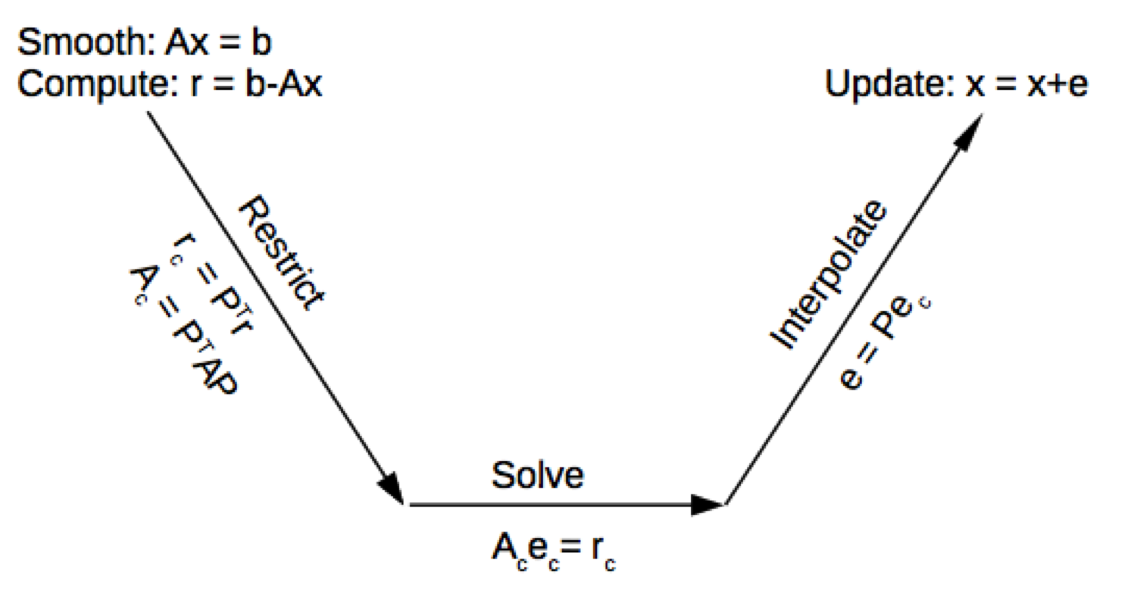
\includegraphics[width=0.7\textwidth]{../figures/TwoGrid.png}
\end{centering}
\end{figure}
\end{frame}


\section{AMG}
\begin{frame}

\textbf{Smoothness:}
$$e^{\mbox{\tiny{T}}}Ae = \lambda \ll 1$$


$$e^{\mbox{\tiny{T}}}Ae = \sum_{i<j} (-a_{ij})(e_i-e_j)^2 \ll 1$$


\textbf{Strength of Connection}
$$-a_{ij}\geq \theta \max_{k\neq i} \{-a_{ik}\} \ \ \ \mbox{where } \theta \in (0,1]$$


\end{frame}


\section{Coarse "grid" selection}


\begin{frame}



Choose grid
\begin{itemize}
  \item[1.] Define strength matrix $A_s$
  \item[2.] Choose set of fine points based on $A_s$
  \item[3.] Choose extra points to satisfy interpolation requirements
\end{itemize}

\vspace{.5in}

\begin{equation} \nonumber
 \wh{\begin{pmatrix}
     -1 &-1&-1\\
     -1 &8&-1\\
     -1 &-1&-1
   \end{pmatrix}}
\end{equation}

\end{frame}


\begin{frame}



Choose grid
\begin{itemize}
  \item[1.] Define strength matrix $A_s$
  \item[2.] Choose set of fine points based on $A_s$
  \item[3.] Choose extra points to satisfy interpolation requirements
\end{itemize}

\vspace{.5in}

FE Poisson stencil:
\begin{equation} \nonumber
 \begin{pmatrix}
     -1 &-1&-1\\
     -1 &8&-1\\
     -1 &-1&-1
   \end{pmatrix}
\end{equation}
\end{frame}

\begin{frame}
% section section_name (end)

\begin{tabular}{ p{0.525\textwidth} p{0.35\textwidth}}

\hspace{5mm} 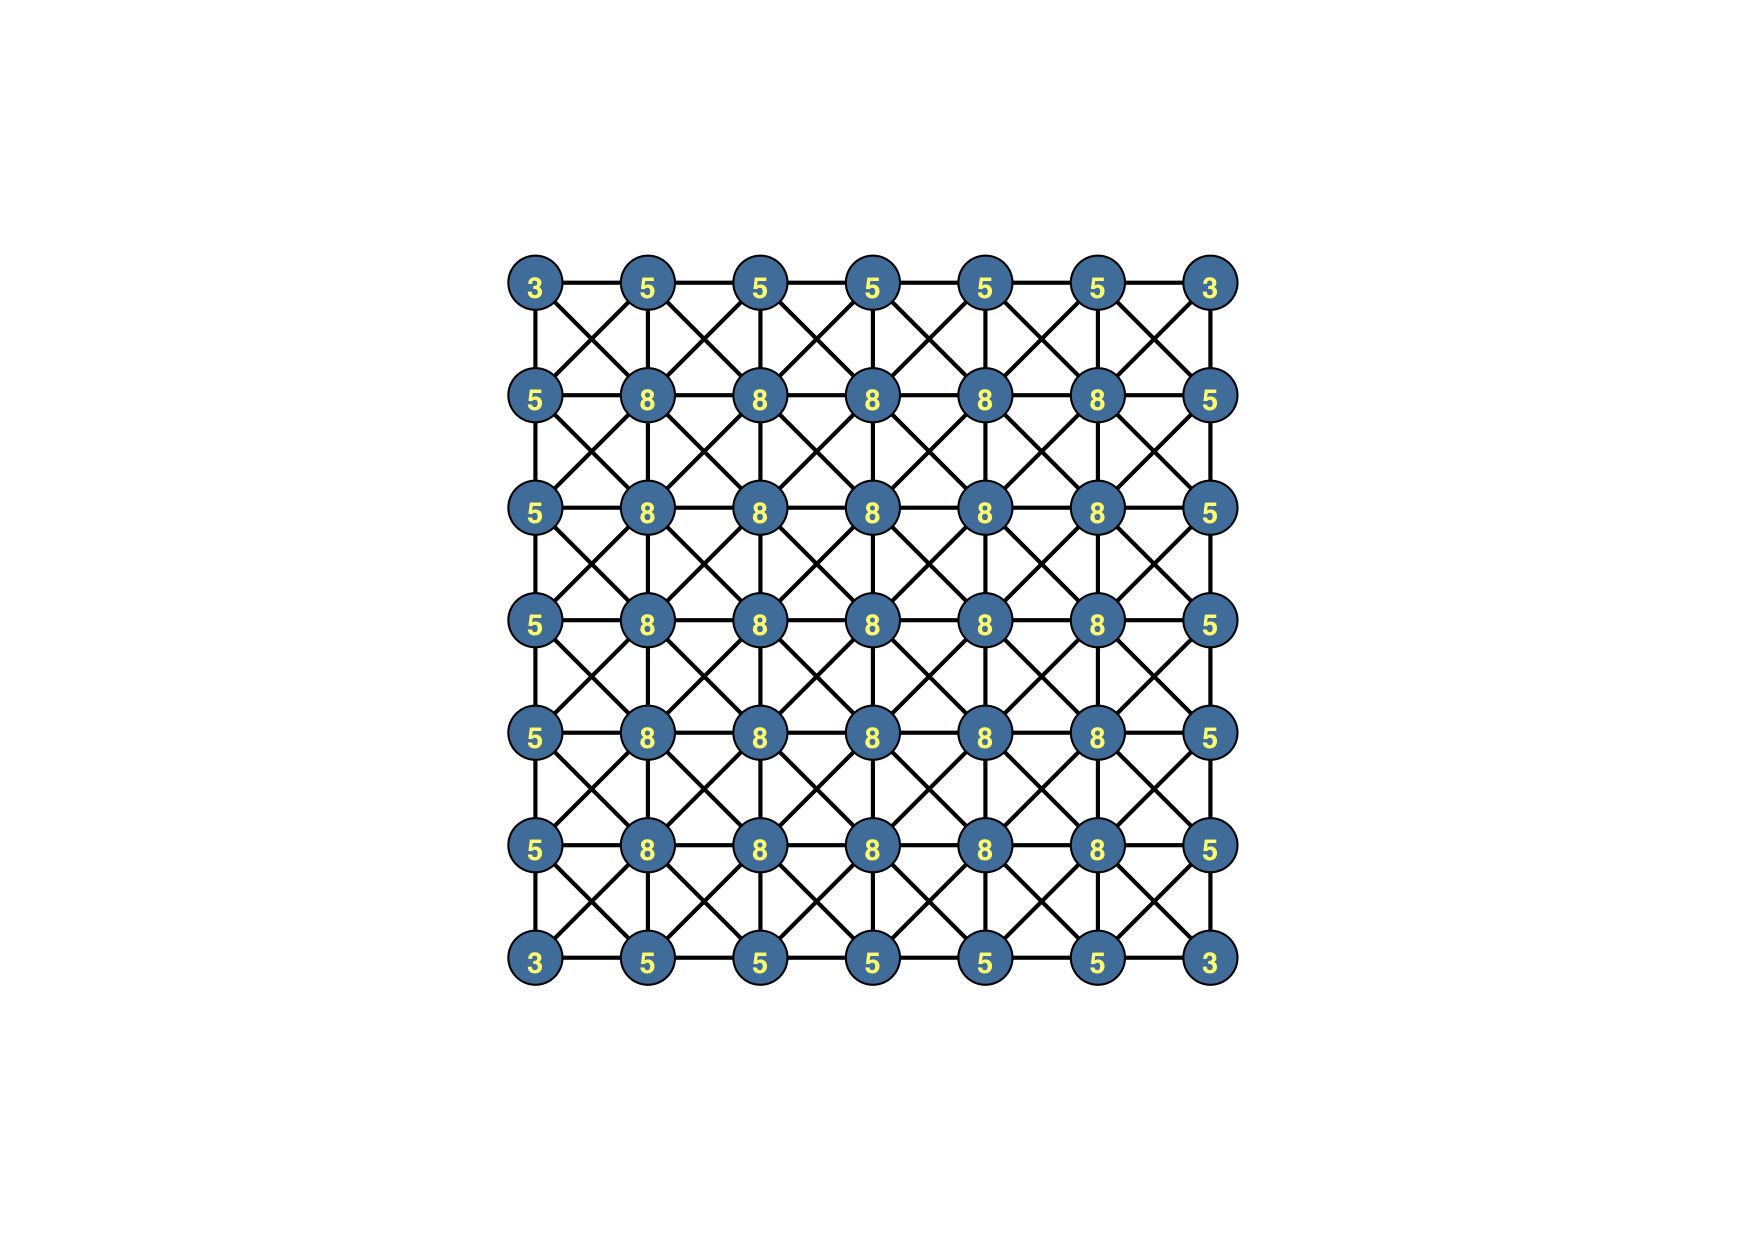
\includegraphics[trim = 85mm 40mm 85mm  40mm, clip, width=0.48\textwidth]{../figures/AMG1.png} &

\vspace{-1.75in}

\begin{itemize}
  \item select C-pt with maximal measure
  \item select neighbours as F-pts
  \item update measures of F-pt neighbours

\end{itemize}

\end{tabular}

\end{frame}

\begin{frame}


\begin{tabular}{ p{0.525\textwidth} p{0.35\textwidth}}

\hspace{5mm} 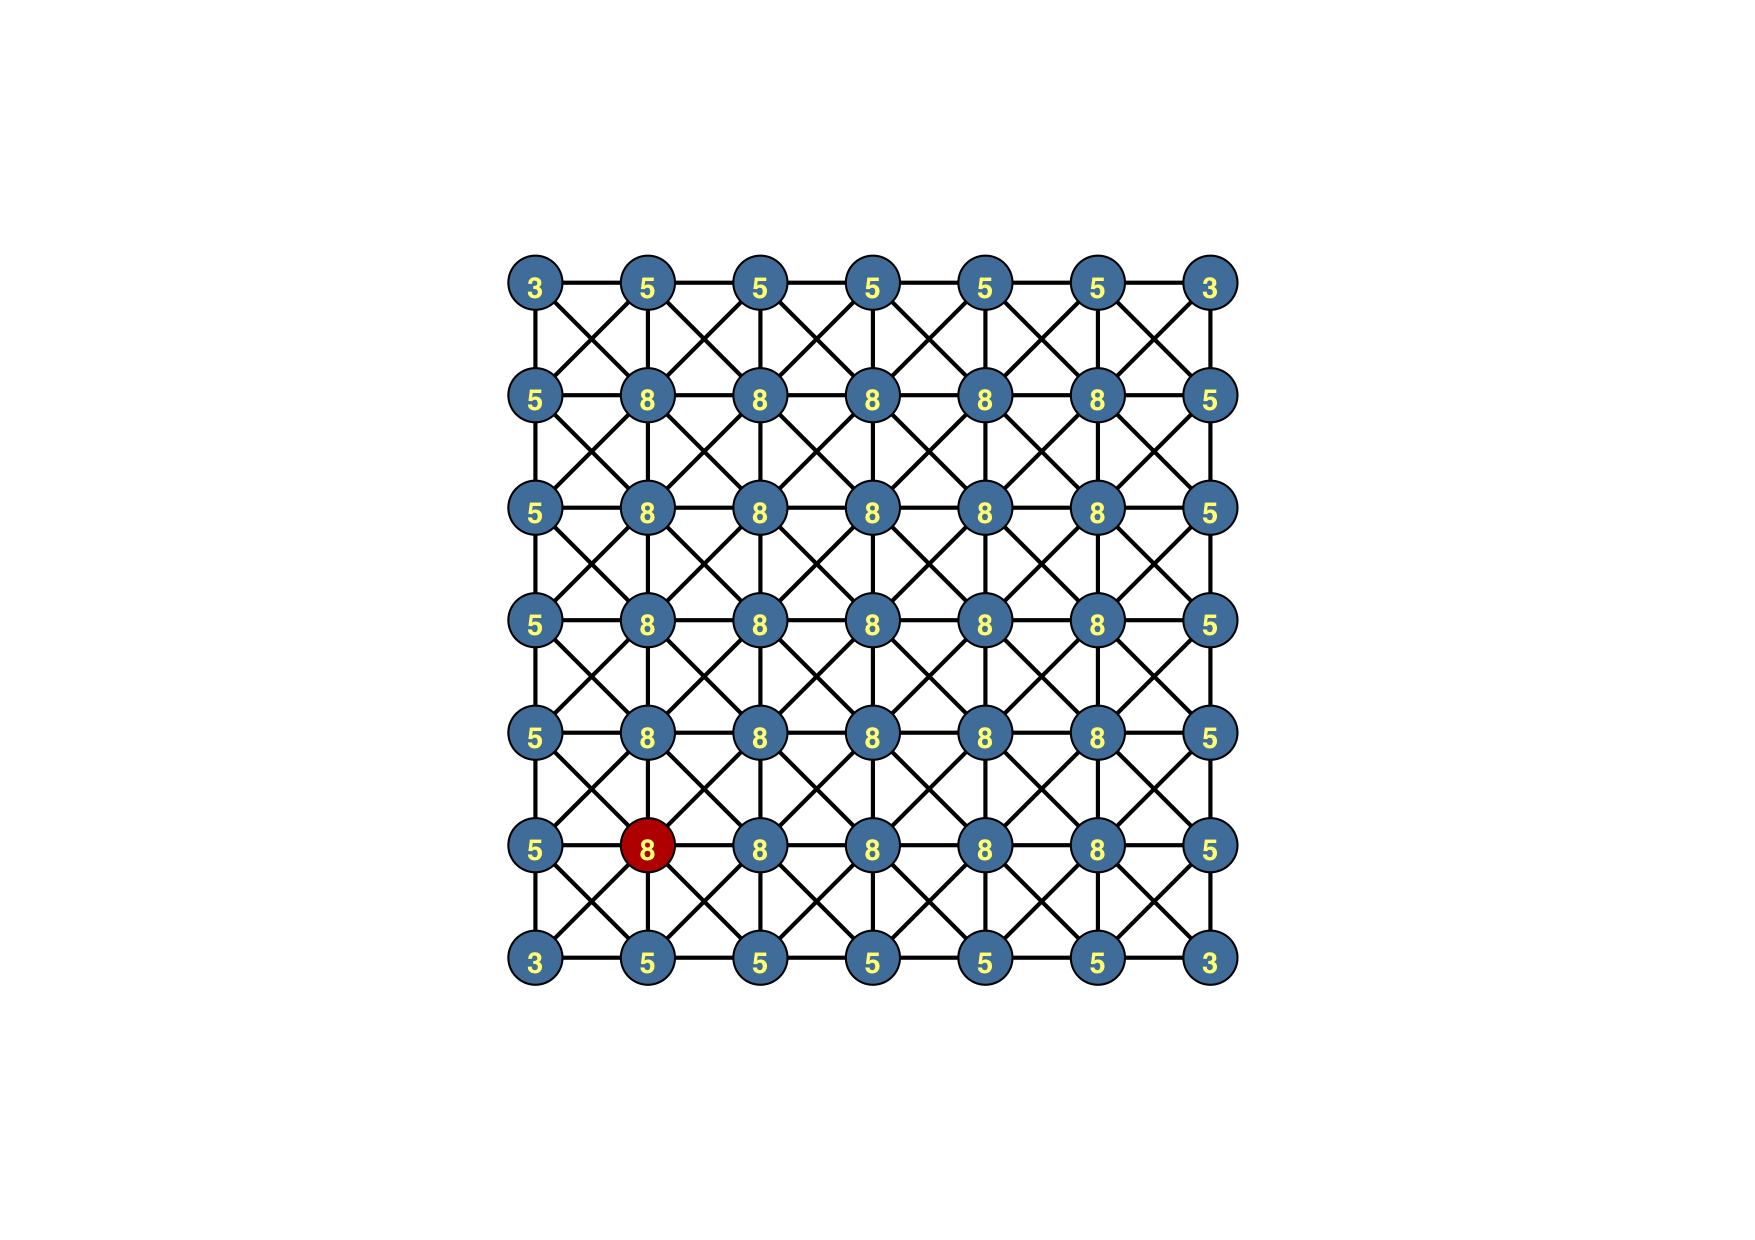
\includegraphics[trim = 85mm 40mm 85mm  40mm, clip, width=0.48\textwidth]{../figures/AMG2.png} &

\vspace{-1.75in}

\begin{itemize}
  \item \re{select C-pt with maximal measure}
  \item select neighbours as F-pts
  \item update measures of F-pt neighbours

\end{itemize}
\end{tabular}

\end{frame}

\begin{frame}


\begin{tabular}{ p{0.525\textwidth} p{0.35\textwidth}}

\hspace{5mm} 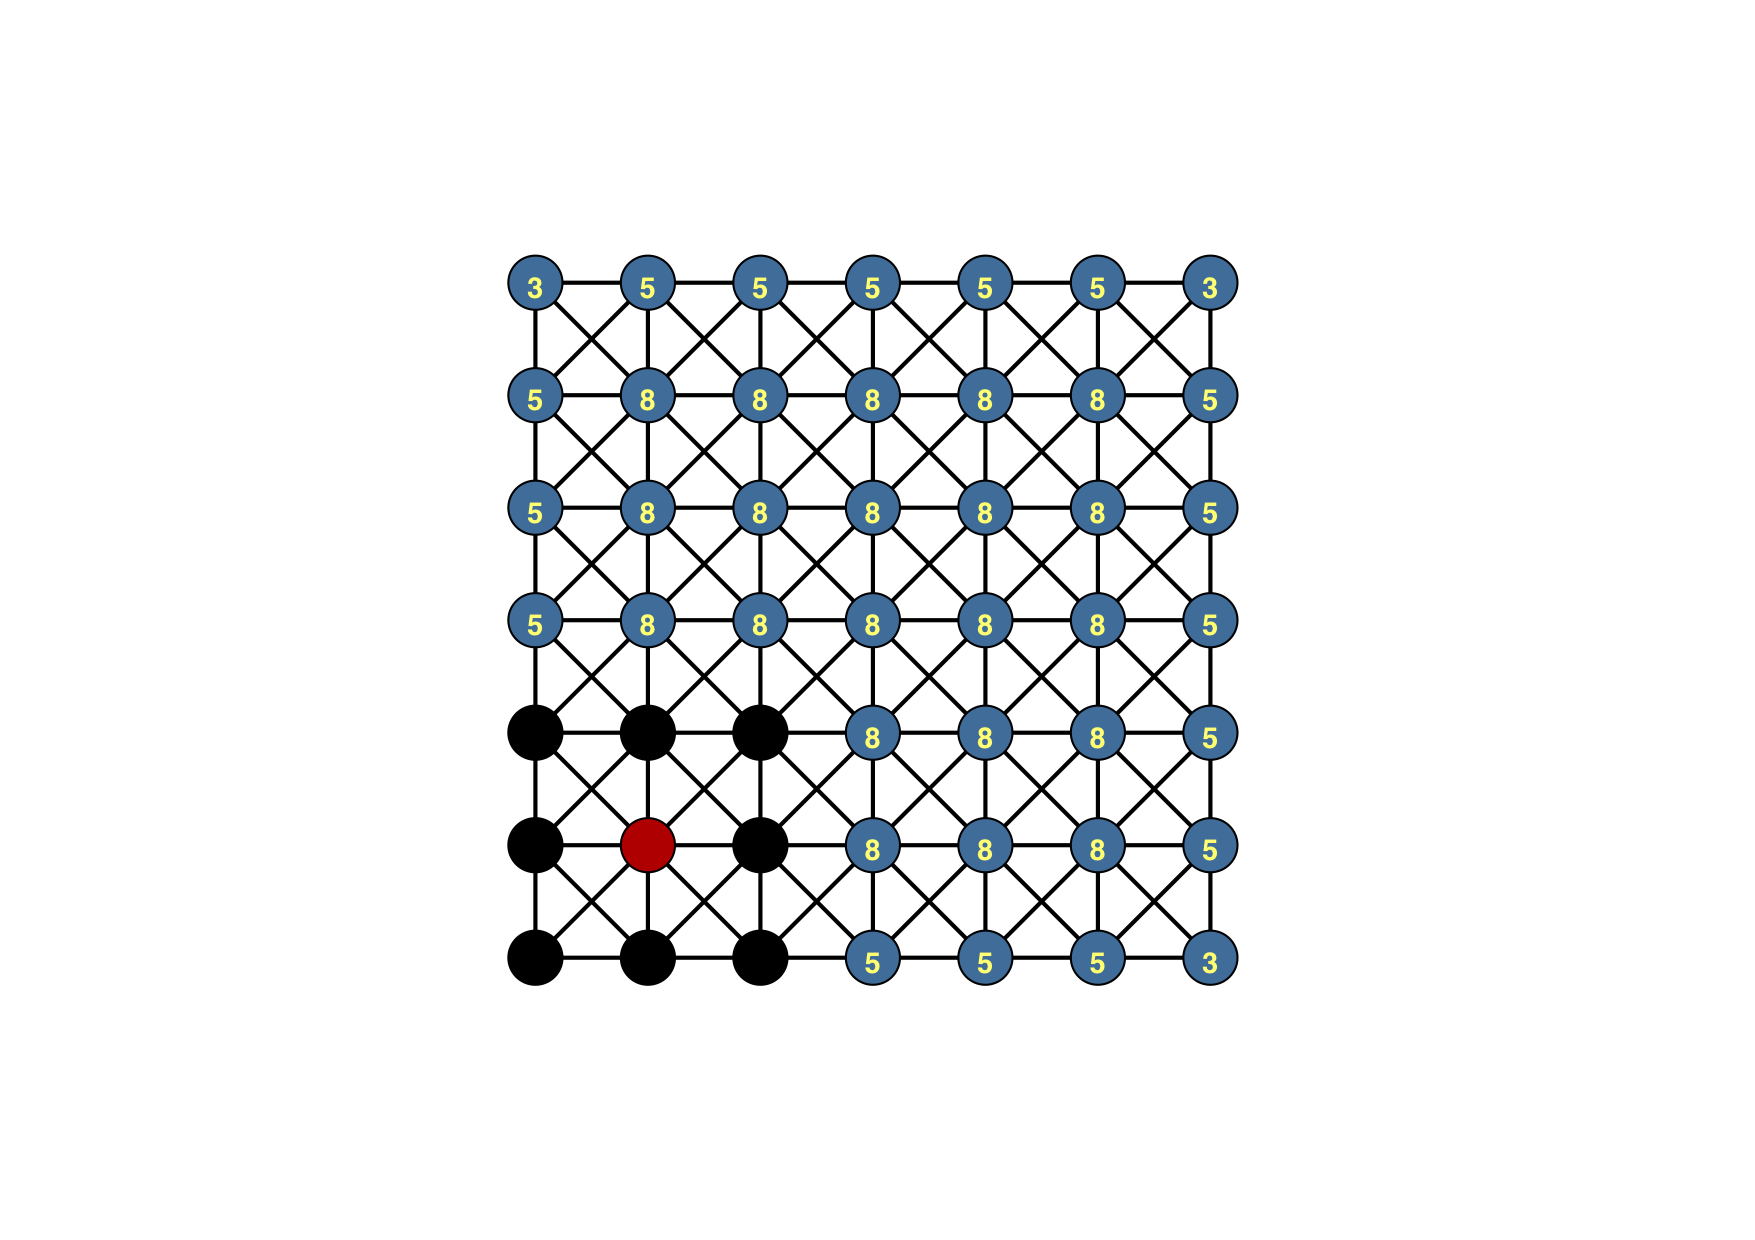
\includegraphics[trim = 85mm 40mm 85mm  40mm, clip, width=0.48\textwidth]{../figures/AMG3.png} &

\vspace{-1.75in}

\begin{itemize}
  \item select C-pt with maximal measure
  \item \re{select neighbours as F-pts}
  \item update measures of F-pt neighbours

\end{itemize}
\end{tabular}


\end{frame}

\begin{frame}


\begin{tabular}{ p{0.525\textwidth} p{0.35\textwidth}}

\hspace{5mm} 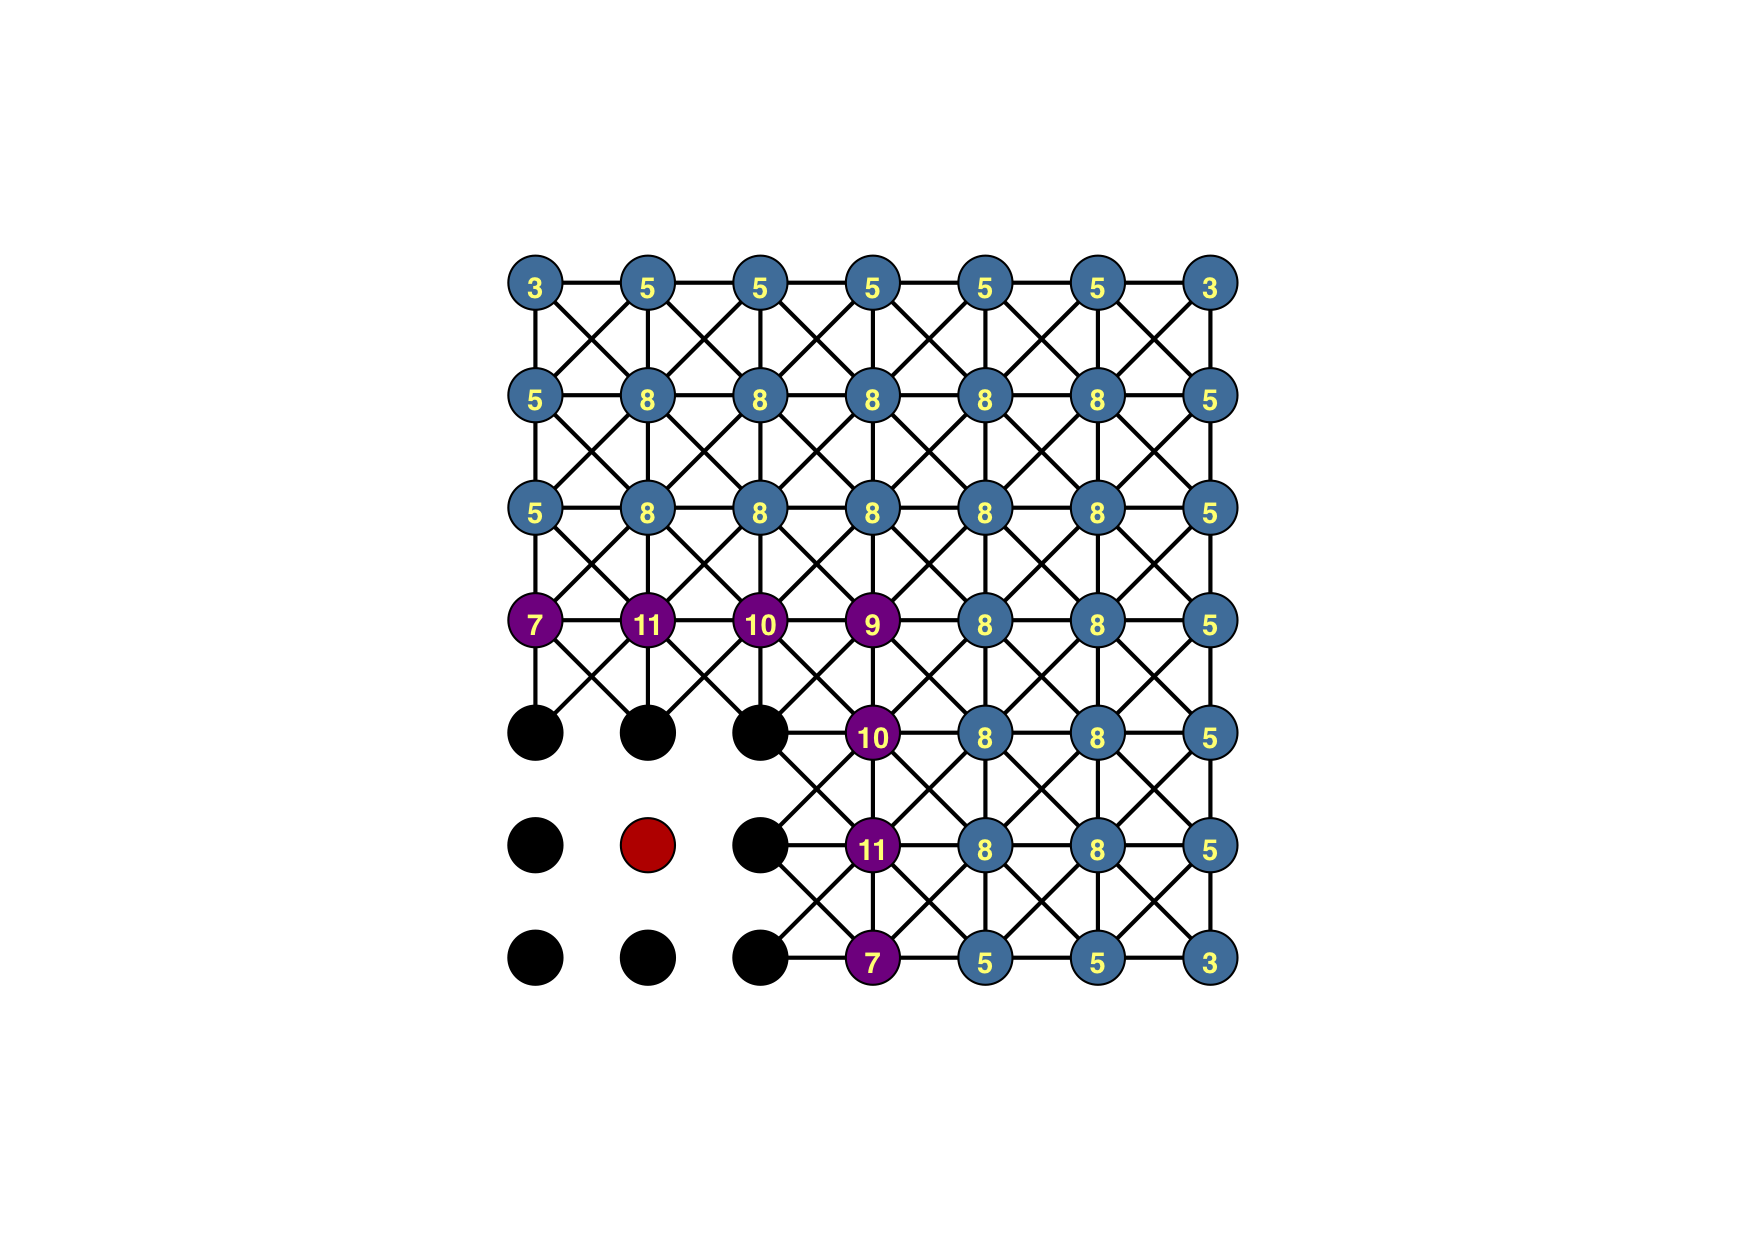
\includegraphics[trim = 85mm 40mm 85mm  40mm, clip, width=0.48\textwidth]{../figures/AMG4.png} &

\vspace{-1.75in}

\begin{itemize}
  \item select C-pt with maximal measure
  \item select neighbours as F-pts
  \item \re{update measures of F-pt neighbours}

\end{itemize}

\end{tabular}

\end{frame}

\begin{frame}



\begin{tabular}{ p{0.525\textwidth} p{0.35\textwidth}}

\hspace{5mm} 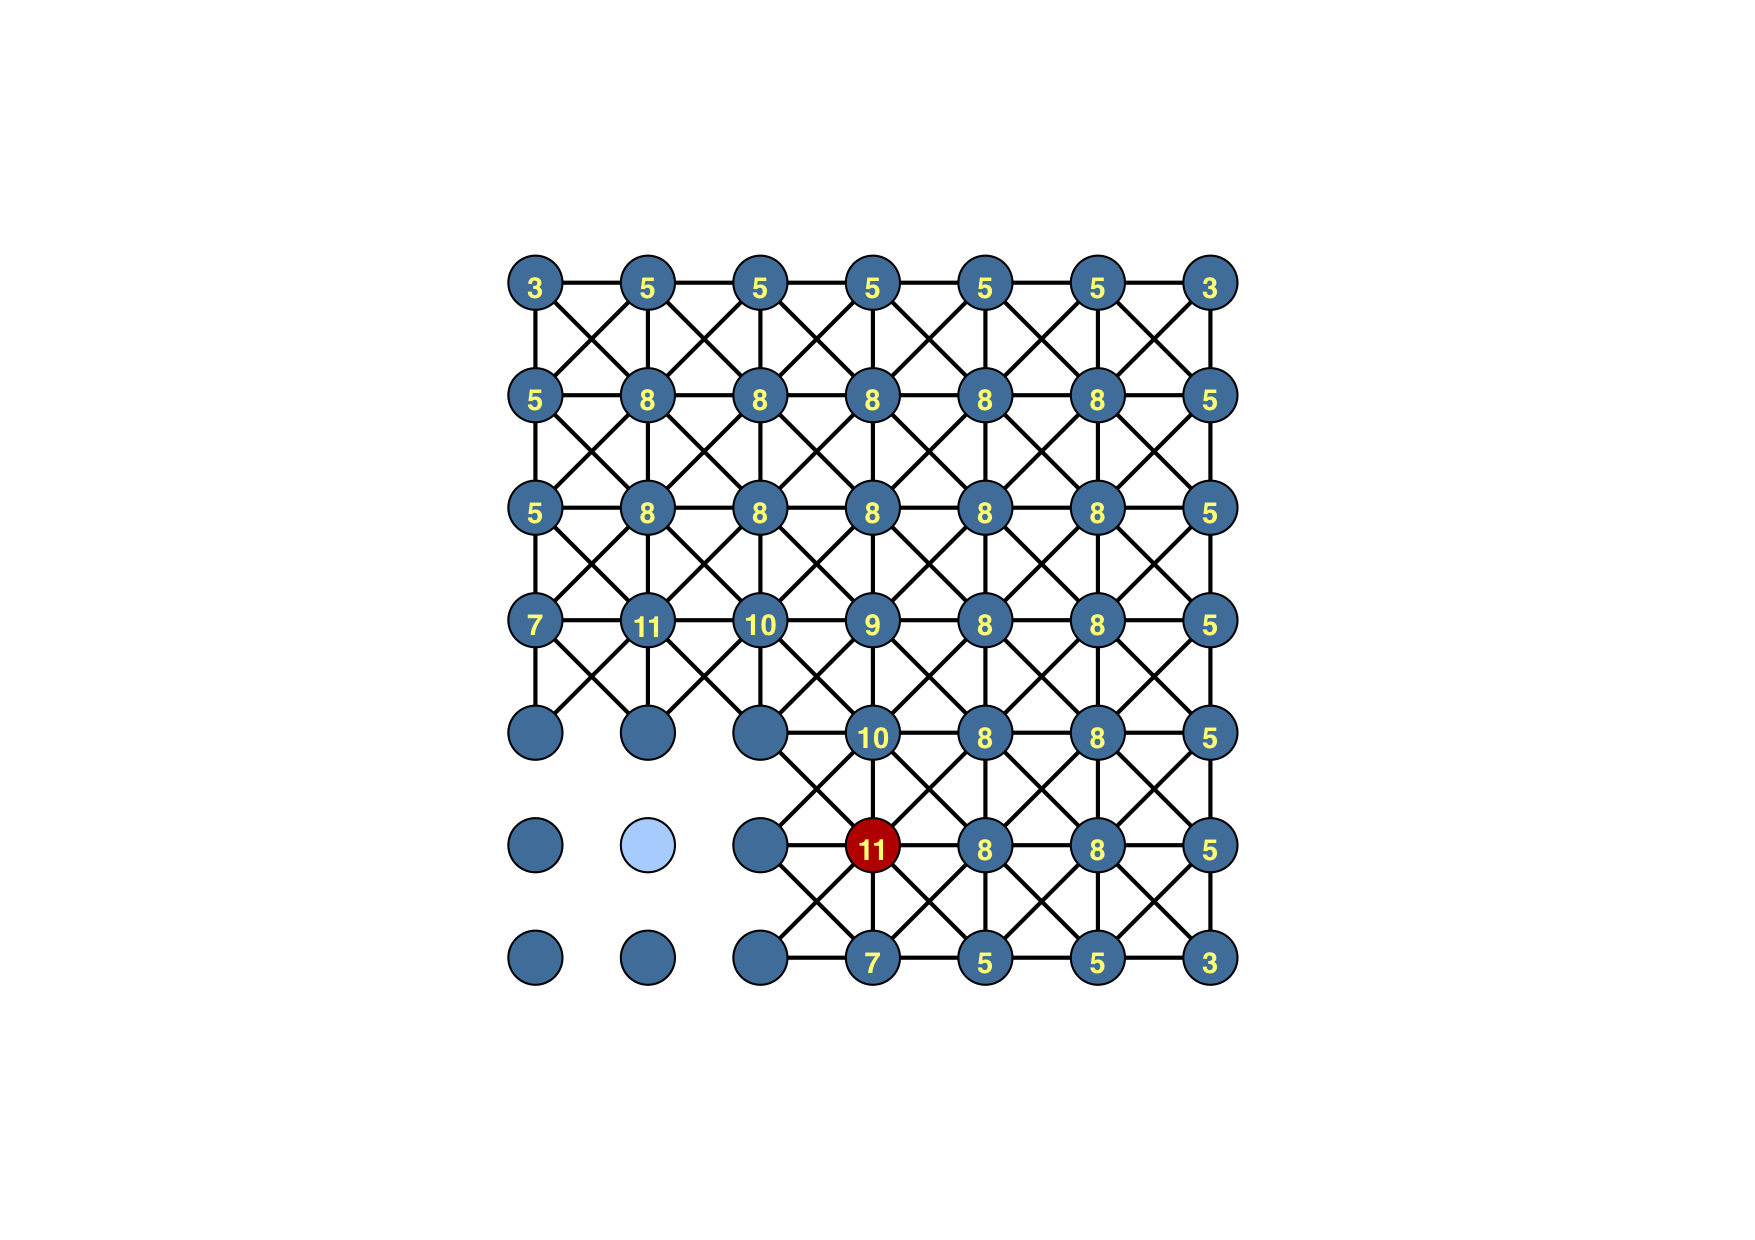
\includegraphics[trim = 85mm 40mm 85mm  40mm, clip, width=0.48\textwidth]{../figures/AMG5.png} &

\vspace{-1.75in}

\begin{itemize}
  \item \re{select C-pt with maximal measure}
  \item select neighbours as F-pts
  \item update measures of F-pt neighbours

\end{itemize}

\end{tabular}

\end{frame}

\begin{frame}



\begin{tabular}{ p{0.525\textwidth} p{0.35\textwidth}}

\hspace{5mm} 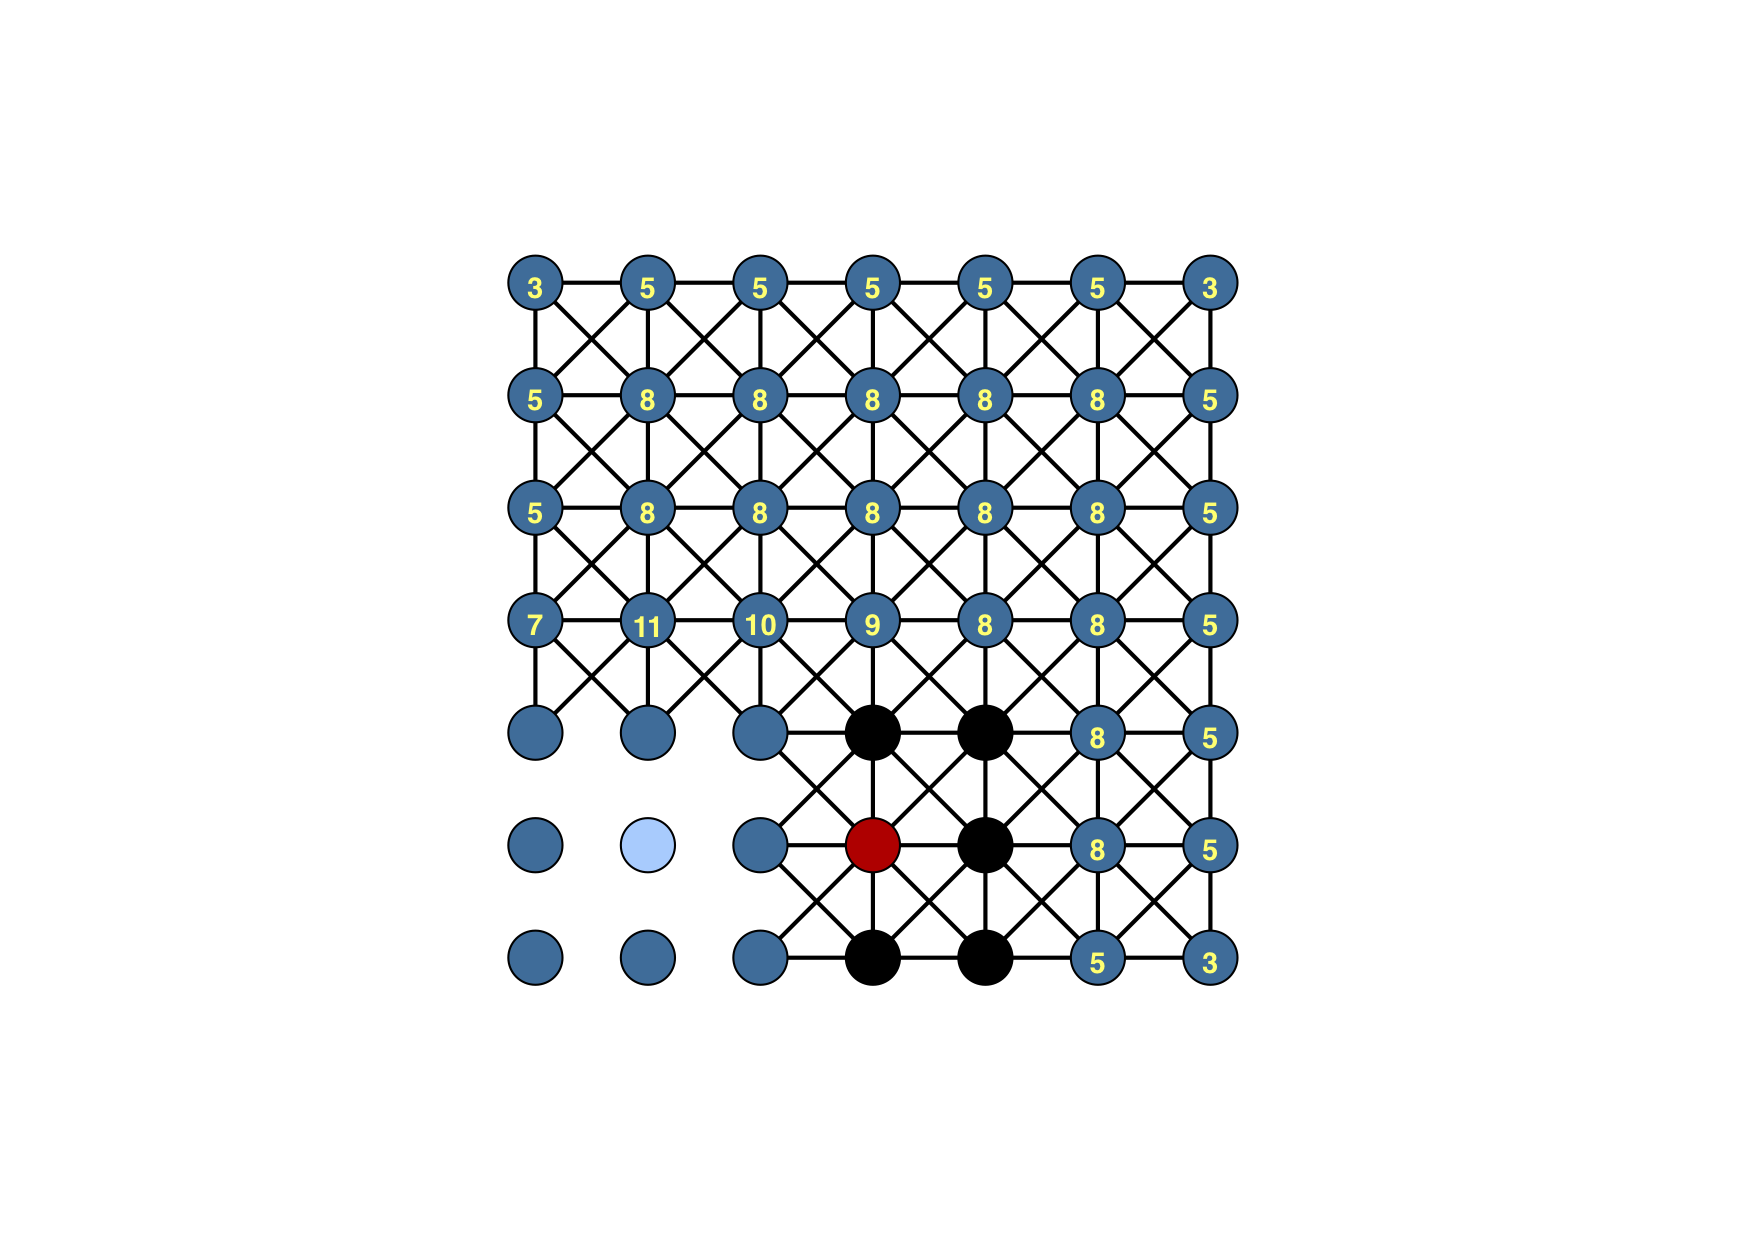
\includegraphics[trim = 85mm 40mm 85mm  40mm, clip, width=0.48\textwidth]{../figures/AMG6.png} &

\vspace{-1.75in}

\begin{itemize}
  \item select C-pt with maximal measure
  \item \re{select neighbours as F-pts}
  \item update measures of F-pt neighbours

\end{itemize}

\end{tabular}

\end{frame}


\begin{frame}


\begin{tabular}{ p{0.525\textwidth} p{0.35\textwidth}}

\hspace{5mm} 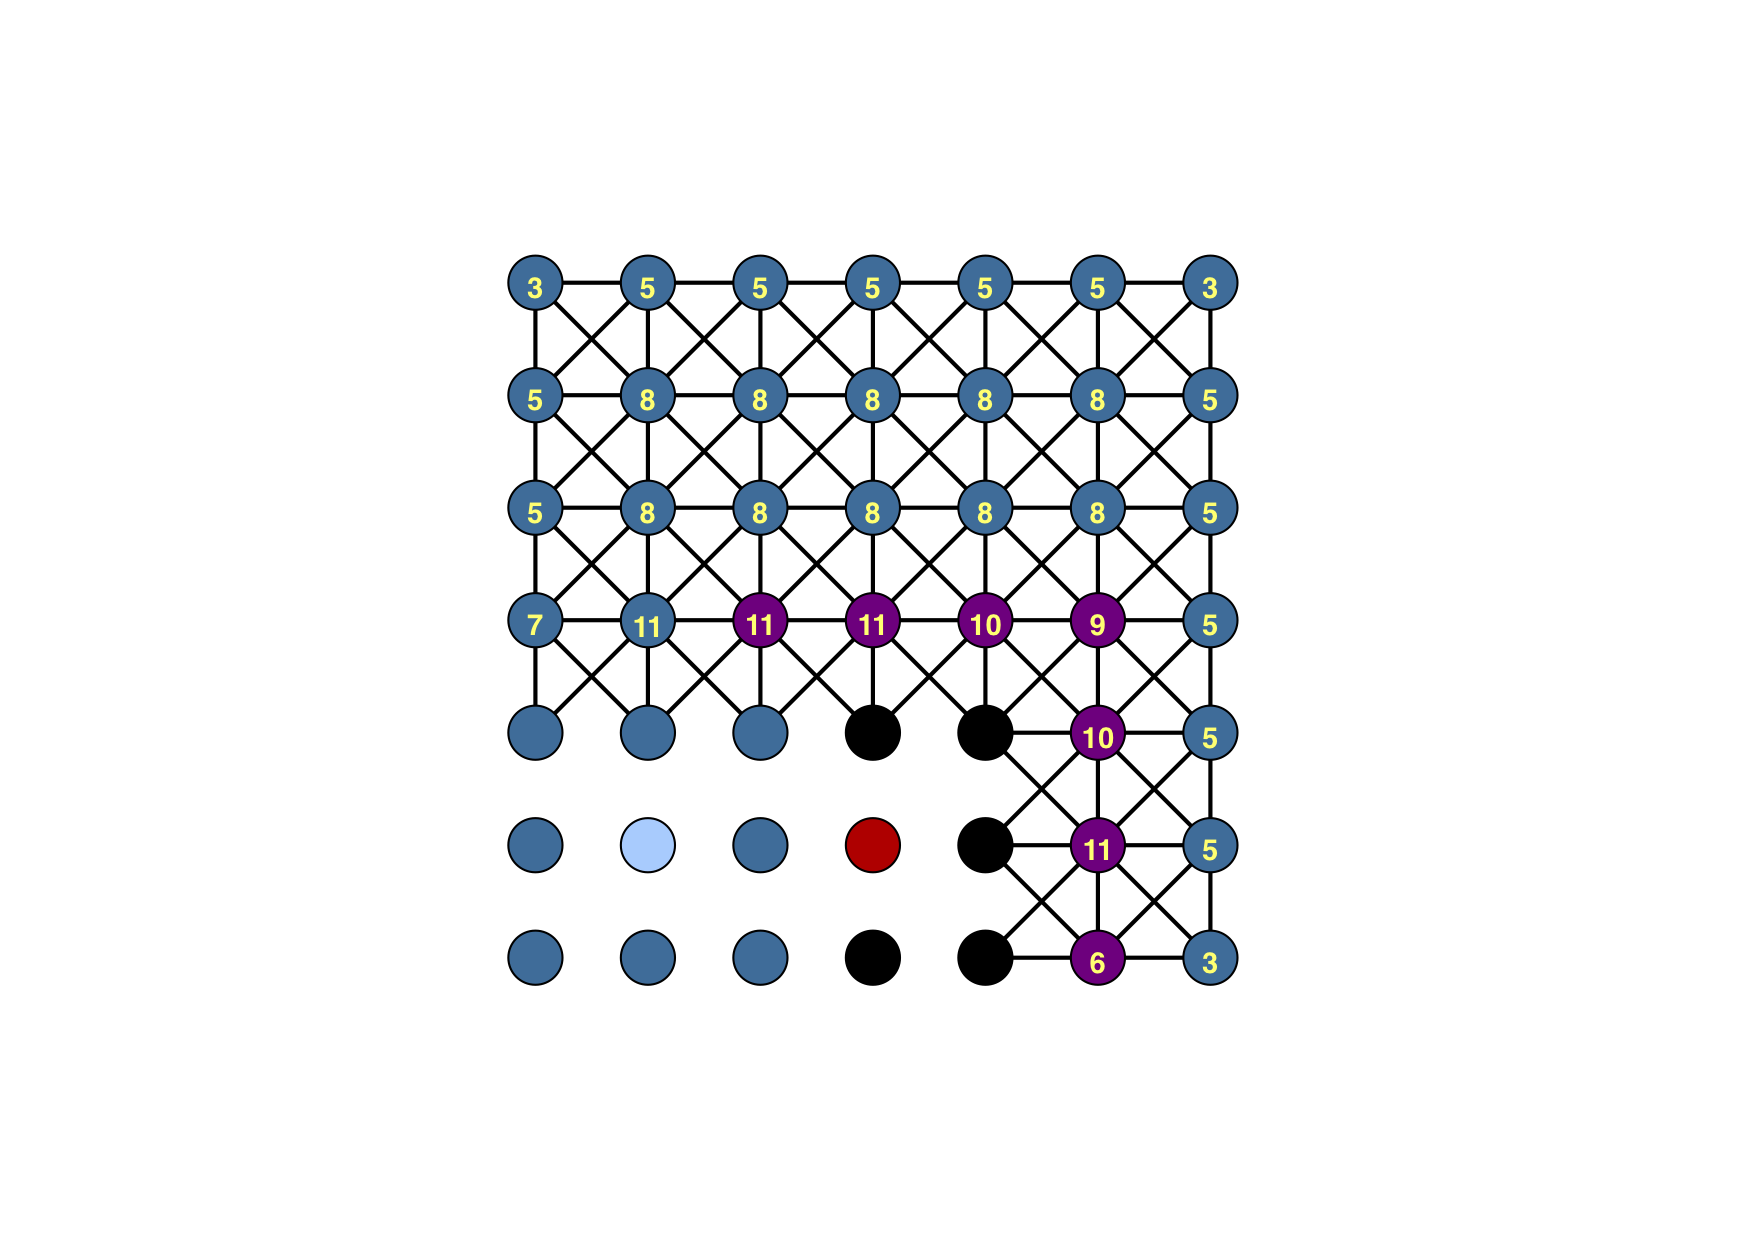
\includegraphics[trim = 85mm 40mm 85mm  40mm, clip, width=0.48\textwidth]{../figures/AMG7.png} &

\vspace{-1.75in}

\begin{itemize}
  \item select C-pt with maximal measure
  \item select neighbours as F-pts
  \item \re{update measures of F-pt neighbours}

\end{itemize}

\end{tabular}

\end{frame}




\begin{frame}



\begin{tabular}{ p{0.525\textwidth} p{0.35\textwidth}}

\hspace{5mm} 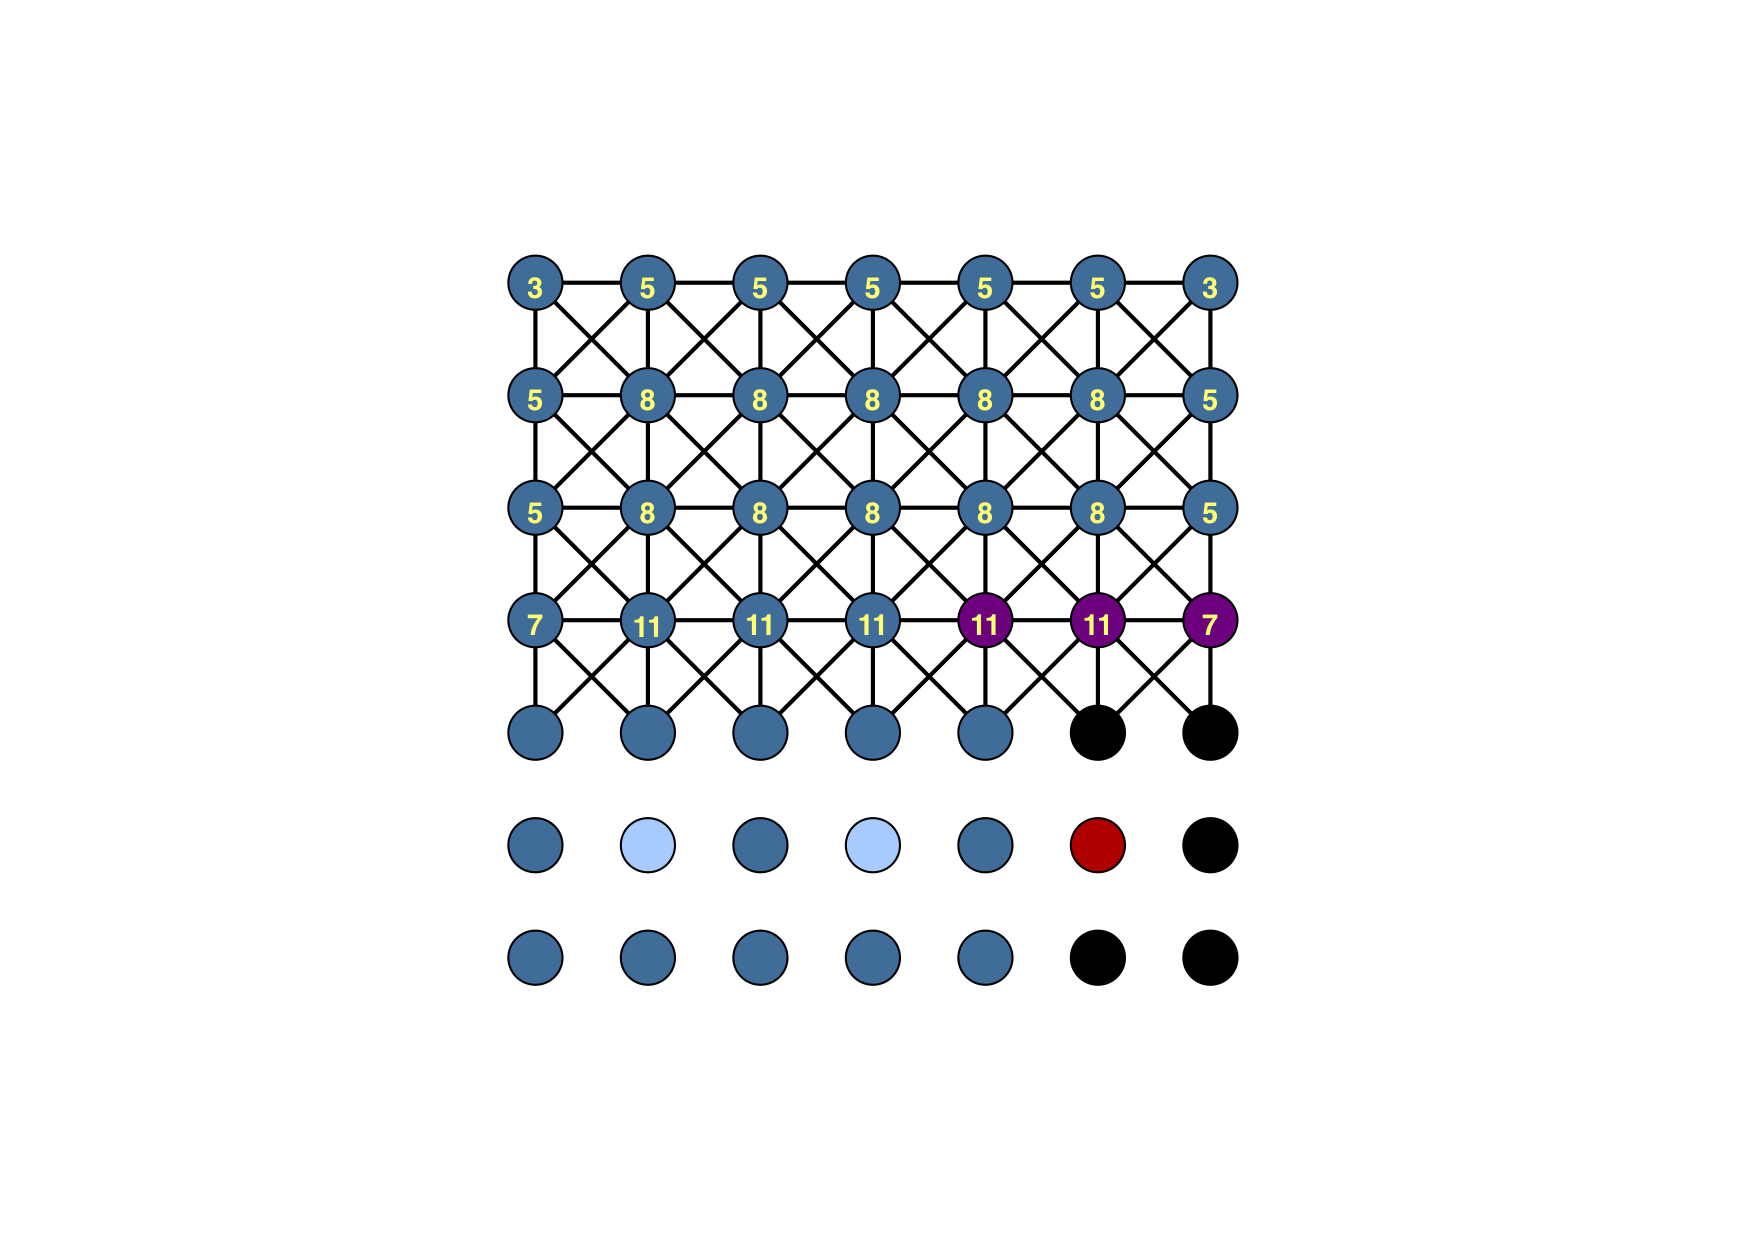
\includegraphics[trim = 85mm 40mm 85mm  40mm, clip, width=0.48\textwidth]{../figures/AMG8.png} &

\vspace{-1.75in}

\begin{itemize}
  \item \re{select C-pt with maximal measure}
  \item \re{select neighbours as F-pts}
  \item \re{update measures of F-pt neighbours}

\end{itemize}

\end{tabular}


\end{frame}


\begin{frame}

\begin{tabular}{ p{0.525\textwidth} p{0.35\textwidth}}

\hspace{5mm} 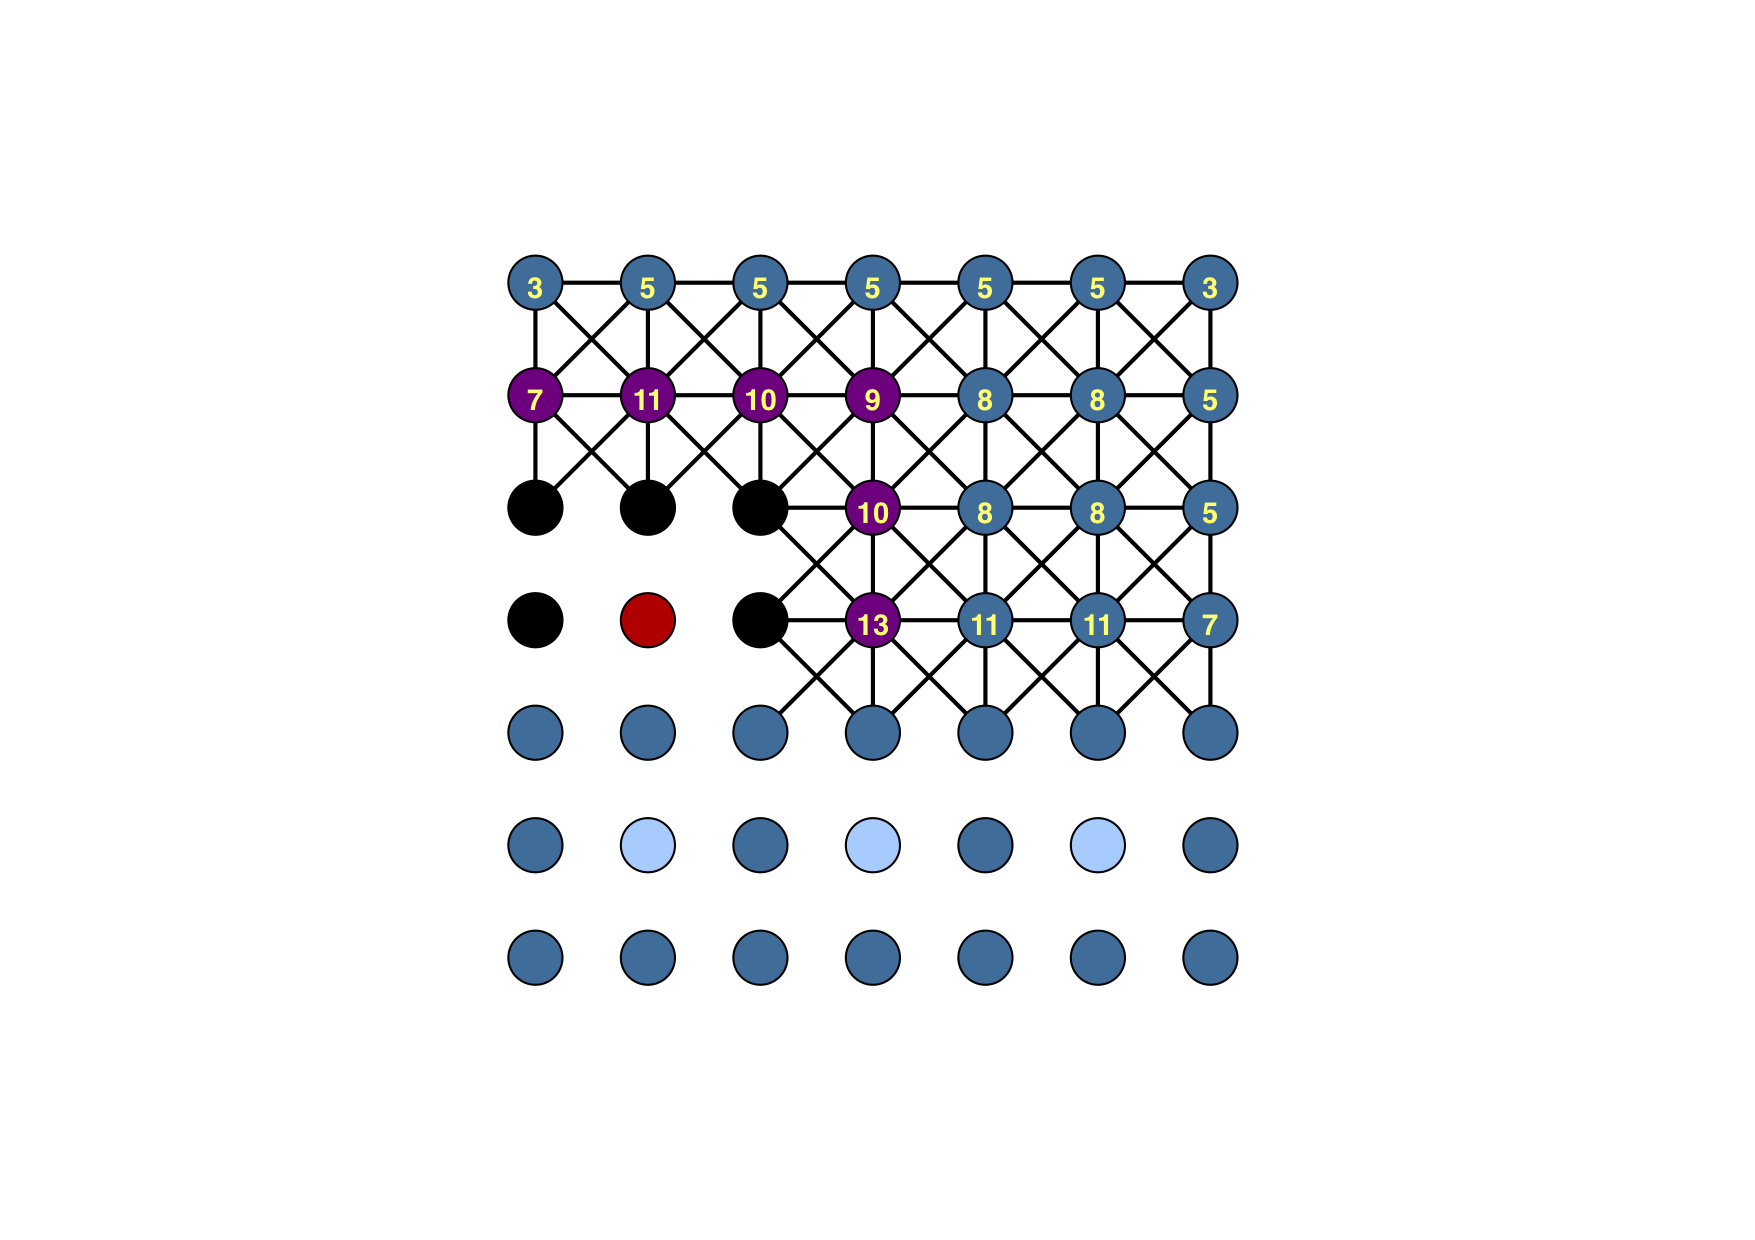
\includegraphics[trim = 85mm 40mm 85mm  40mm, clip, width=0.48\textwidth]{../figures/AMG9.png} &

\vspace{-1.75in}

\begin{itemize}
  \item \re{select C-pt with maximal measure}
  \item \re{select neighbours as F-pts}
  \item \re{update measures of F-pt neighbours}

\end{itemize}

\end{tabular}


\end{frame}


\begin{frame}


\begin{tabular}{ p{0.525\textwidth} p{0.35\textwidth}}

\hspace{5mm} 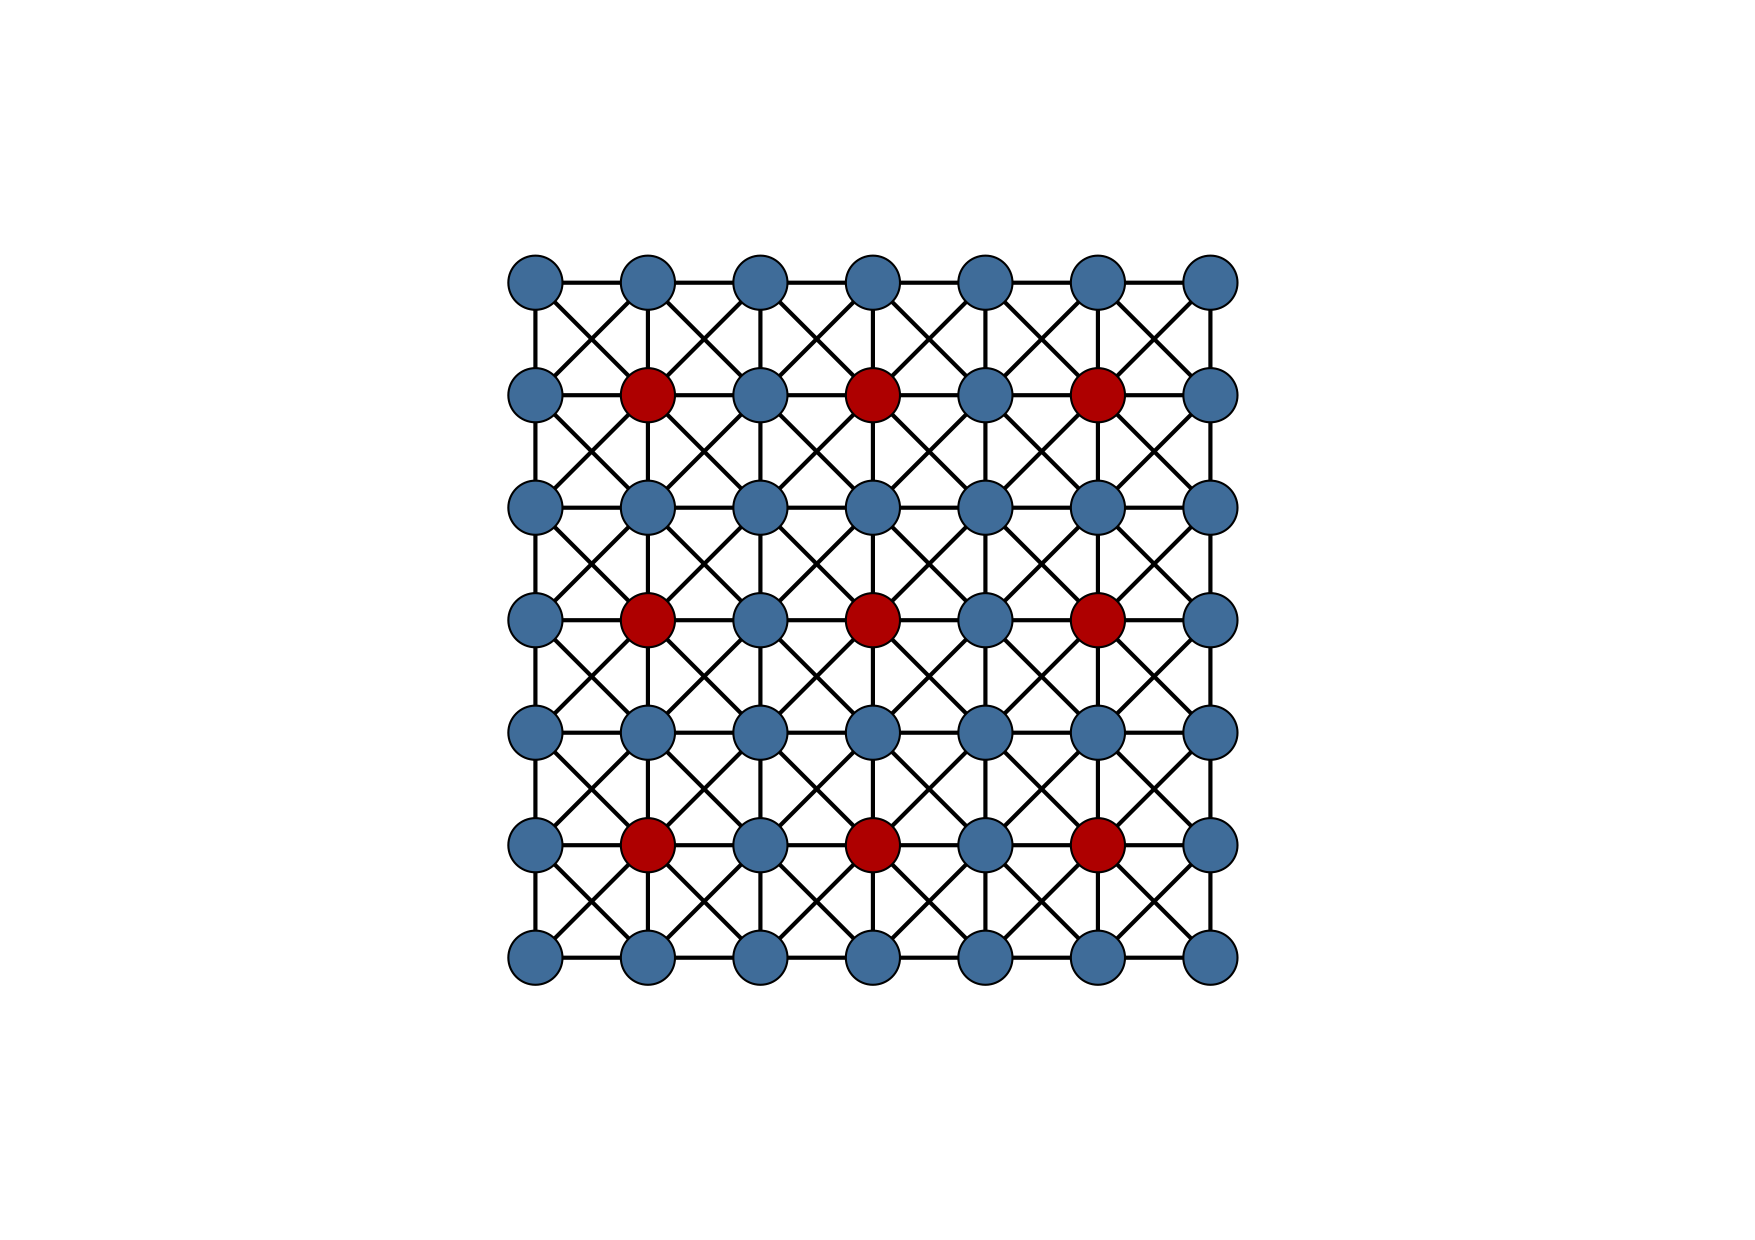
\includegraphics[trim = 85mm 40mm 85mm  40mm, clip, width=0.48\textwidth]{../figures/AMG10.png} &

\vspace{-1.75in}

\begin{itemize}
  \item select C-pt with maximal measure
  \item select neighbours as F-pts
  \item update measures of F-pt neighbours

\end{itemize}

\end{tabular}
\tiny{Falgout (2006)}
\end{frame}



\begin{frame}
\textbf{Second pass}

Classical AMG:
\begin{itemize}
  \item Loop though F-points
  \item find pairs of F-points that are strongly connected
  \item check F-point pair strongly connected to C-point
\end{itemize}


\begin{picture}(1000,40)
\put(150,30){\vector(-1,-1){40}}
\put(150,30){\vector(1,-1){40}}
\end{picture}


\vspace{-.35in} \hspace{1.5in}yes \hspace{.65in} no

\vspace{.3in}
\begin{table}[H]
% \centering
\begin{tabular}{p{0.25\textwidth} p{0.1\textwidth} p{0.2\textwidth}}
% \begin{center}
check next F-point pair & &\hspace{-.4in} make one F-point a C-point
% \end{center}
\end{tabular}
\end{table}

\end{frame}

\section{Interpolate}


\begin{frame}
\frametitle{Interpolate}

\textbf{Smooth error:}
$$\lambda^2 = e^{\mbox{\tiny T}}A^{\mbox{\tiny T}} Ae = r^{\mbox{\tiny T}}r = ||r|| \ll1$$
\textbf{Derive interpolation:}
$$r_i = (Ae)_i = 0$$

    $$a_{ii}e_i = -\sum_{j\in C_i} a_{ij}e_j -\sum_{j\in F_i} a_{ij} e_j -\sum_{j\in N_i} a_{ij}e_j $$

$C_i$: C-points strongly connected to $ i$

$F_i$: F-points strongly connected to $i$

$N_i$: all points weakly connected to $i$

\end{frame}



\begin{frame}
\frametitle{Collapse stencil}

\begin{figure}[h!]
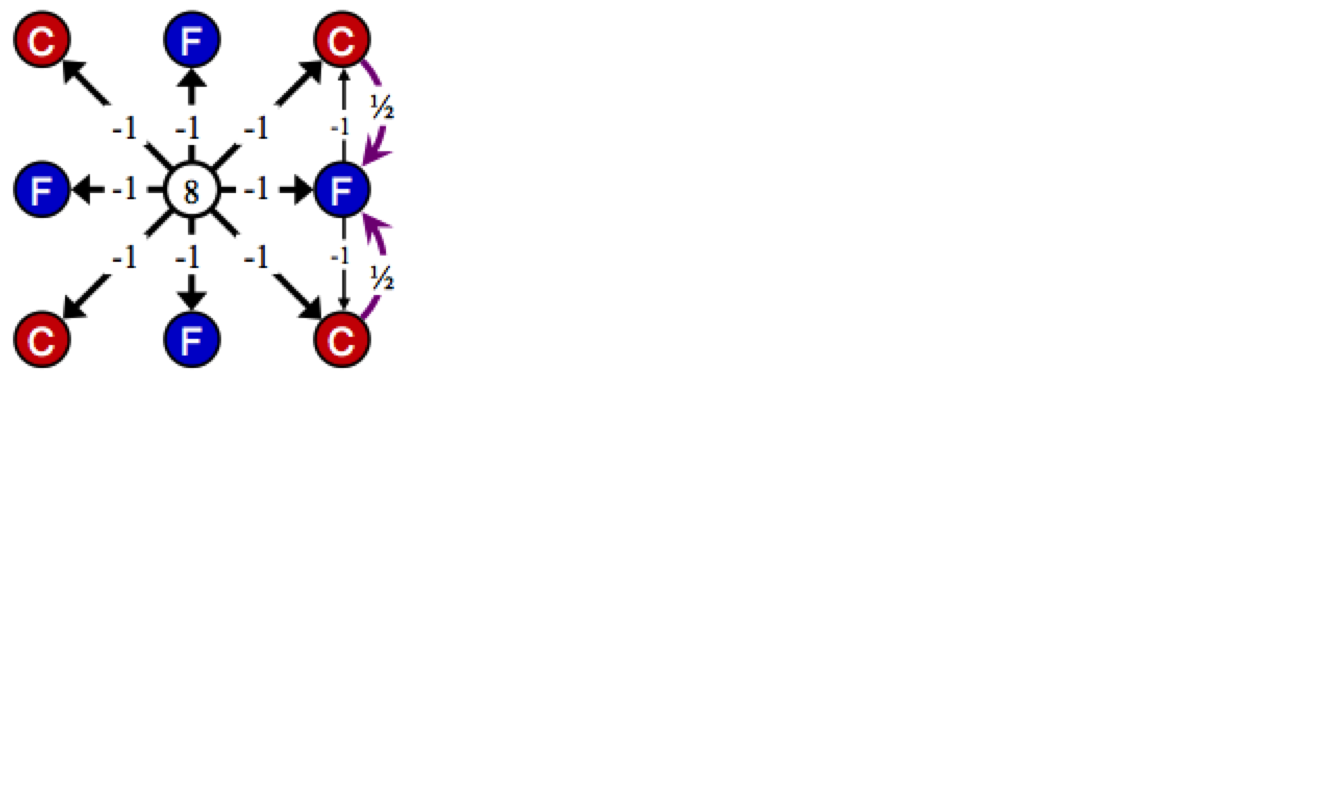
\includegraphics[width=3.2in]{../figures/step1.png}
\end{figure}

\end{frame}


\begin{frame}

\frametitle{Collapse stencil}


\begin{figure}[h!]
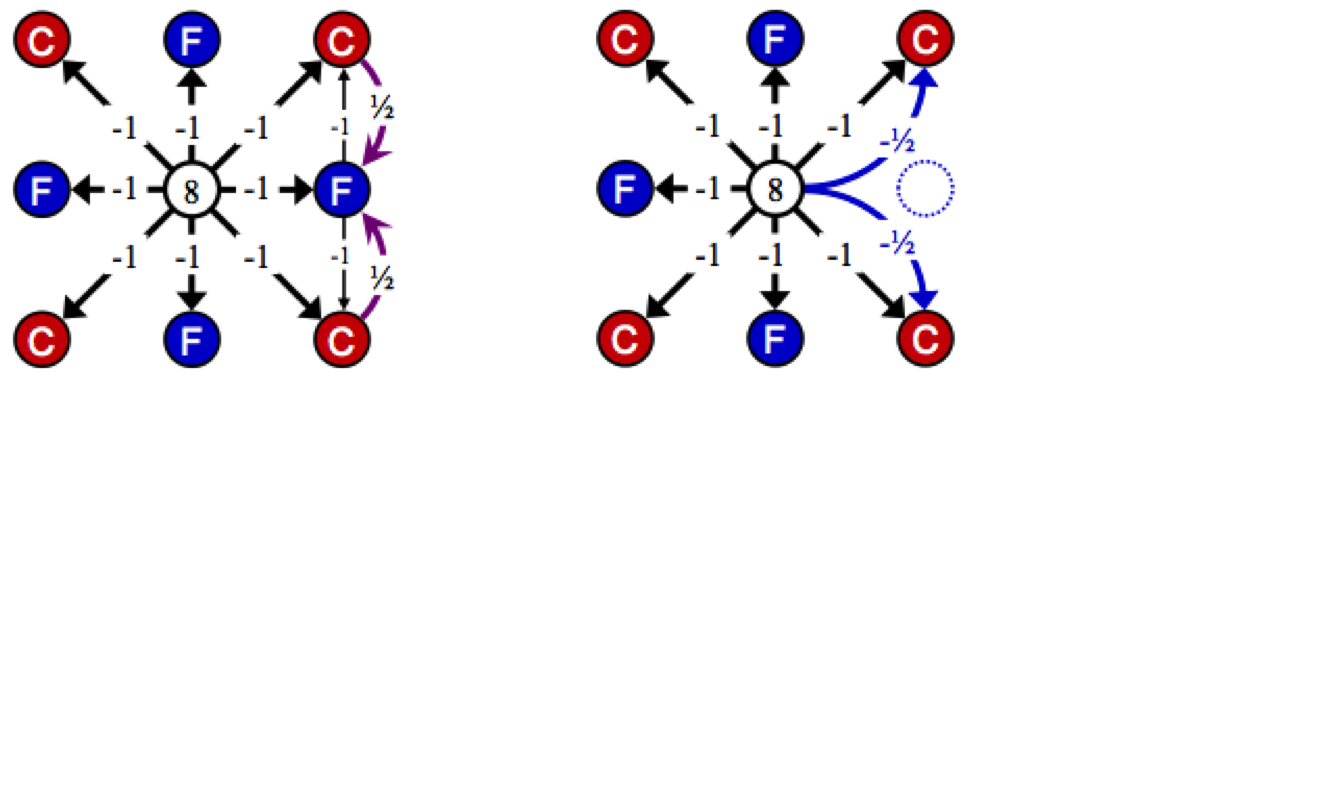
\includegraphics[width=3.2in]{../figures/step2.png}
\end{figure}


\end{frame}


\begin{frame}

\frametitle{Collapse stencil}


\begin{figure}[h!]
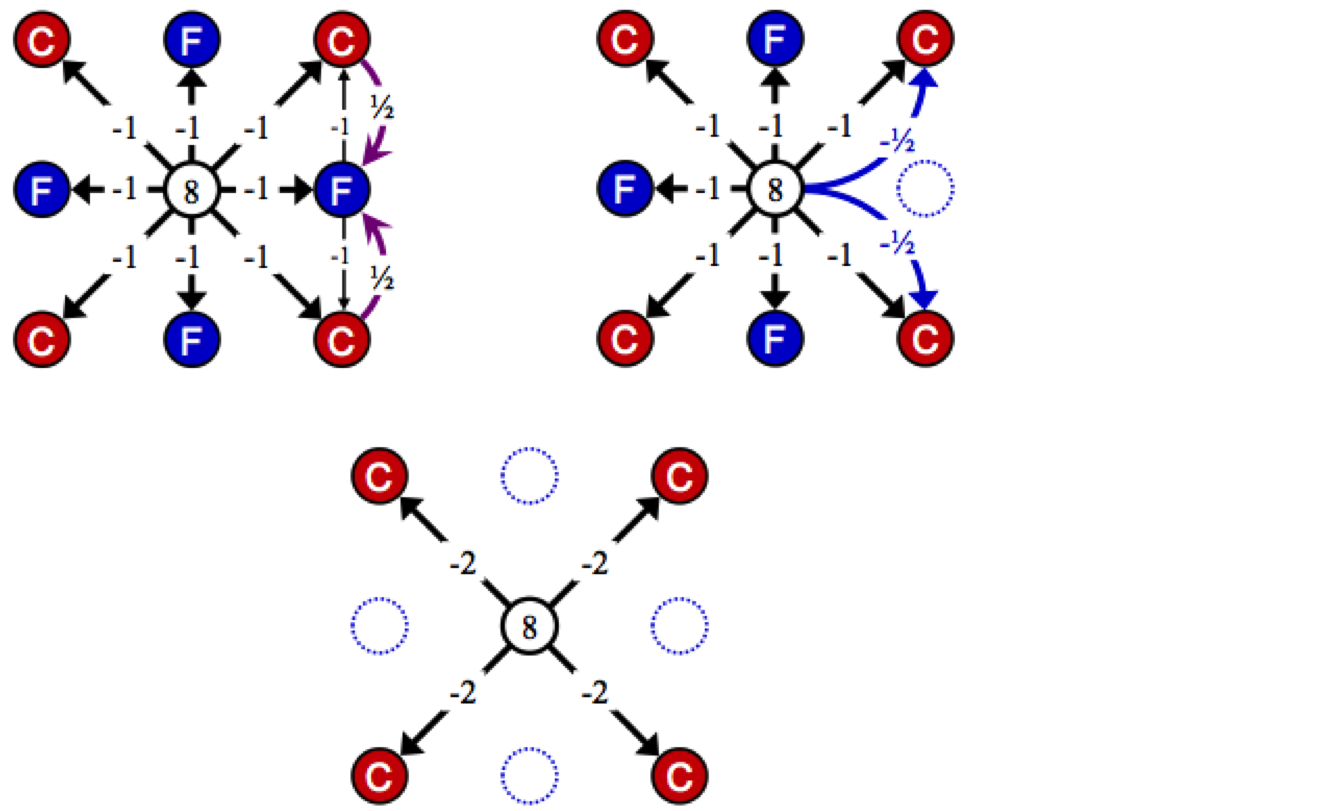
\includegraphics[width=3.2in]{../figures/step3.png}
\end{figure}

\end{frame}


\begin{frame}

\frametitle{Collapse stencil}


\begin{figure}[h!]
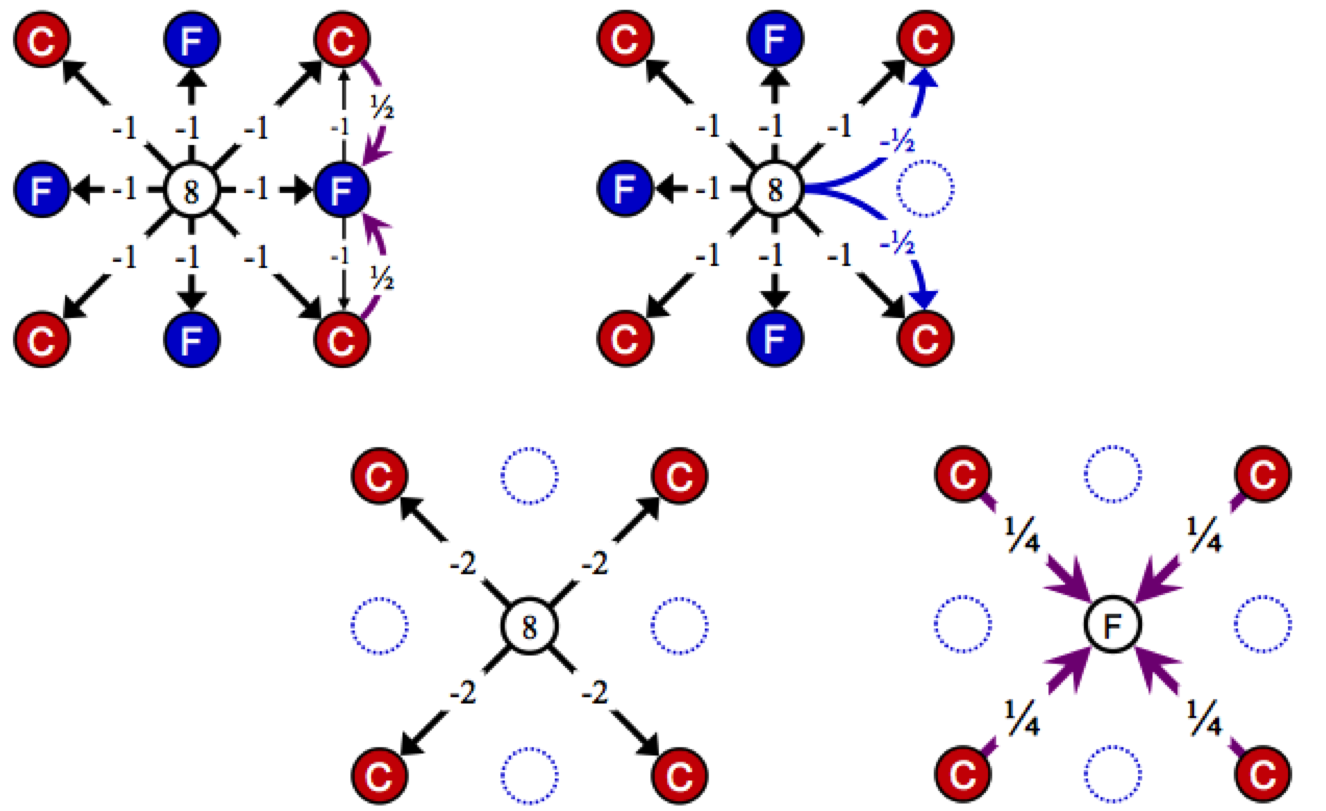
\includegraphics[width=3.2in]{../figures/step4.png}
\end{figure}

\tiny{Falgout (2006)}
\end{frame}


\section{Example}
\begin{frame}
\vspace{-.3in}
\frametitle{Poisson}
\begin{equation} \nonumber
    \begin{aligned}
      \re{  -\Delta \vec u }& \re{= \vec f} \ \ \ \mbox{in } \Omega \\
         \re{\vec u} &\re{= \vec 0} \ \ \ \mbox{on } \partial\Omega
    \end{aligned}
\end{equation}


{\footnotesize
\begin{tabular}{rrrrrrr}
\hline
 Grid  &      DoF & \multicolumn{2}{c}{AMG} & \multicolumn{2}{c}{ILU}& Direct (MUMPS)  \\

  size &       &  $\#$ iters &  Soln Time &  $\#$ iters &  Soln Time &     Soln Time \\

\hline

       $   2  ^2$&       18 &        1 &   1.31e-05 &                 1 &   6.91e-06 &   5.29e-04 \\
       $   4  ^2$&       50 &        2 &   3.60e-05 &                 5 &   1.22e-05 &   4.99e-04 \\
       $   8  ^2$&      162 &        3 &   1.25e-04 &                8 &   5.41e-05 &   8.80e-04 \\
       $  16  ^2$&      578 &        4 &   5.80e-04 &              14 &   1.96e-04 &   2.89e-03 \\
       $  32  ^2$&     2178 &        4 &   1.94e-03 &             25 &   1.38e-03 &   9.74e-03 \\
       $  64  ^2$&     8450 &        4 &   7.73e-03 &             48 &   1.06e-02 &   6.84e-02 \\
       $ 128 ^2$ &    33282 &        4 &   3.01e-02 &           93 &   7.92e-02 &   3.38e-01 \\
       $ 256 ^2$ &   132098 &        4 &   1.36e-01 &         181 &   6.99e-01 &   1.77e+00 \\
       $ 512 ^2$ &   526338 &        4 &   6.05e-01 &         349 &   5.81e+00 &   9.76e+00 \\
       $1024^2$ &  2101250 &        4 &   2.49e+00 &       668 &   4.62e+01 &   6.33e+01 \\
      $2048^2$ &  8396802 &        4 &       9.98e+00 &          1272 &     3.47e+02 &         5.66e+02 \\
% 6 &     $ 128^3$ &  6440067 &        6 &   2.09e+01 \\
\hline
\end{tabular}

}


\end{frame}

\begin{frame}

\textbf{3 Dimensional example}

\vspace{.1in}

{\footnotesize
\begin{tabular}{rrrrrrr}
\hline

 Grid  &      DoF & \multicolumn{2}{c}{AMG} & \multicolumn{2}{c}{ILU}& Direct (MUMPS)  \\

  size &       &  $\#$ iters &  Soln Time &  $\#$ iters &  Soln Time &     Soln Time \\

\hline
    %   2 &       81 &        1 &   1.69e-05 &           1 &   7.87e-06 &       0 \\
    %   4 &      375 &        2 &   1.16e-04 &           4 &   3.60e-05 &       0 \\
    %   8 &     2187 &        3 &   1.35e-03 &         8 &   3.84e-04 &       0 \\
    %  16 &    14739 &        3 &   1.22e-02 &       14 &   5.53e-03 &        0 \\
    %  32 &   107811 &        3 &   1.26e-01 &      26 &   8.82e-02 &        0 \\
    %  64 &   823875 &        4 &   1.63e+00 &     45 &   1.31e+00&          0 \\
    % 128 &  6440067 &        4 &   1.60e+01 &  84 &   1.94e+01 &        0 \\


  $  2  ^3$ &      81 &        1 &   1.81e-05 &             1 &   7.87e-06 &   7.22e-04 \\
  $  4  ^3$ &     375 &        2 &   1.19e-04 &            4 &   3.60e-05 &   1.50e-03 \\
  $  8  ^3$ &    2187 &        3 &   1.37e-03 &             8 &   3.85e-04 &    9.22e-03 \\
  $ 16 ^3$  &   14739 &        3 &   1.24e-02 &        14 &   5.35e-03 &    2.44e-01 \\
  $ 32 ^3$  &  107811 &        3 &   1.26e-01 &         26 &   8.98e-02 &   1.29e+01 \\
  $ 64 ^3$  &   823875 &        4 &   1.63e+00 &     45 &   1.31e+00&          1.04e+03 \\
  $128^3$    &  6440067 &        4 &   1.60e+01 &  84 &   1.94e+01 &        - \\


% 6 &     $ 128^3$ &  6440067 &        6 &   2.09e+01 \\
\hline
\end{tabular}

}

\end{frame}

\section{Conclusion}
\begin{frame}
\frametitle{Summary}


\begin{itemize}
  \item Tries to mimic GMG

  \vspace{.15in}

  \item Relies on matrix coefficients

  \vspace{.15in}

  \item No geometric information needed

  \vspace{.15in}

  \item Black box for elliptic problems
\end{itemize}

\end{frame}

% \begin{frame}
% \begin{equation} \nonumber
%     \begin{aligned}
%       \re{  -\nu \Delta \vec u+ \nabla p} \ & \re{= \vec f} \\
%          \re{ \div \vec u   } \ & \re{= 0 }\\
%         % \vec u &= \vec 0 \ \ \ \mbox{on } \partial\Omega}
%     \end{aligned} \ \ \ \ \  \mbox{in } \Omega \hspace{24mm}
% \end{equation}
% \vspace{-3mm}
% \begin{equation} \nonumber
% \mbox{\hspace{-1.5mm}} \re{\vec u = \vec g} \ \ \ \ \ \ \mbox{on } \partial\Omega
% \end{equation}

% Viscosity $ \re{\nu}$, velocity $ \re{\vec u}$ and pressure $ \re{p}$

% \end{frame}

% \begin{frame}

% \frametitle{Stokes}

% $$ \re{\mathcal{K} = \begin{bmatrix}
% A & B^{\mbox{\tiny{T}}}\\
% B & 0\\
% \end{bmatrix} \hspace{15mm}
% \mathcal{M} = \begin{bmatrix}
% A & 0\\
%  0& M\\
% \end{bmatrix}}
% $$

% \end{frame}
\nocite{*}

\bibliographystyle{apalike}
{\footnotesize
\bibliography{ref}}

\end{document}